%!TEX root = ../mieic.tex

\chapter{Revisão Bibliográfica} \label{chap:chap2}

\section*{}

\section{Introdução}

Esta dissertação foca-se mais na forma como se apresenta o conteúdo que se pretende recomendar ao utilizador, e não qual o conteúdo que é sugerido (não obstante da sua importância obviamente).
No entanto, é quase impossível, no estudo do estado da arte, não se refirir outros projetos que se focam também no conteúdo.
Nesse sentido, será feita uma pequena análise dos conteúdos sugeridos.
Regra geral, os projetos que de seguida serão analisados, utilizam bases de dados externas, como o last.fm, para obter metadata que, convenientemente, também oferecem um tipo de recomendação de música com base numa pesquisa inicial.

\section{Projetos Relacionados} % (fold)
\label{sec:projetos_relacionados}


\subsection{liveplasma.com} % (fold)
\label{sub:projeto_1}

O liveplasma.com é uma aplicação em flash que mosta relações de artistas de música em forma de grafo, para além de também permitir criar grafos com livros e filmes.
Este não permite editar o grafo e, ao clicar num nó o grafo, é novamente gerado apartir desse nó.

\begin{figure}[tb]
  \begin{center}
    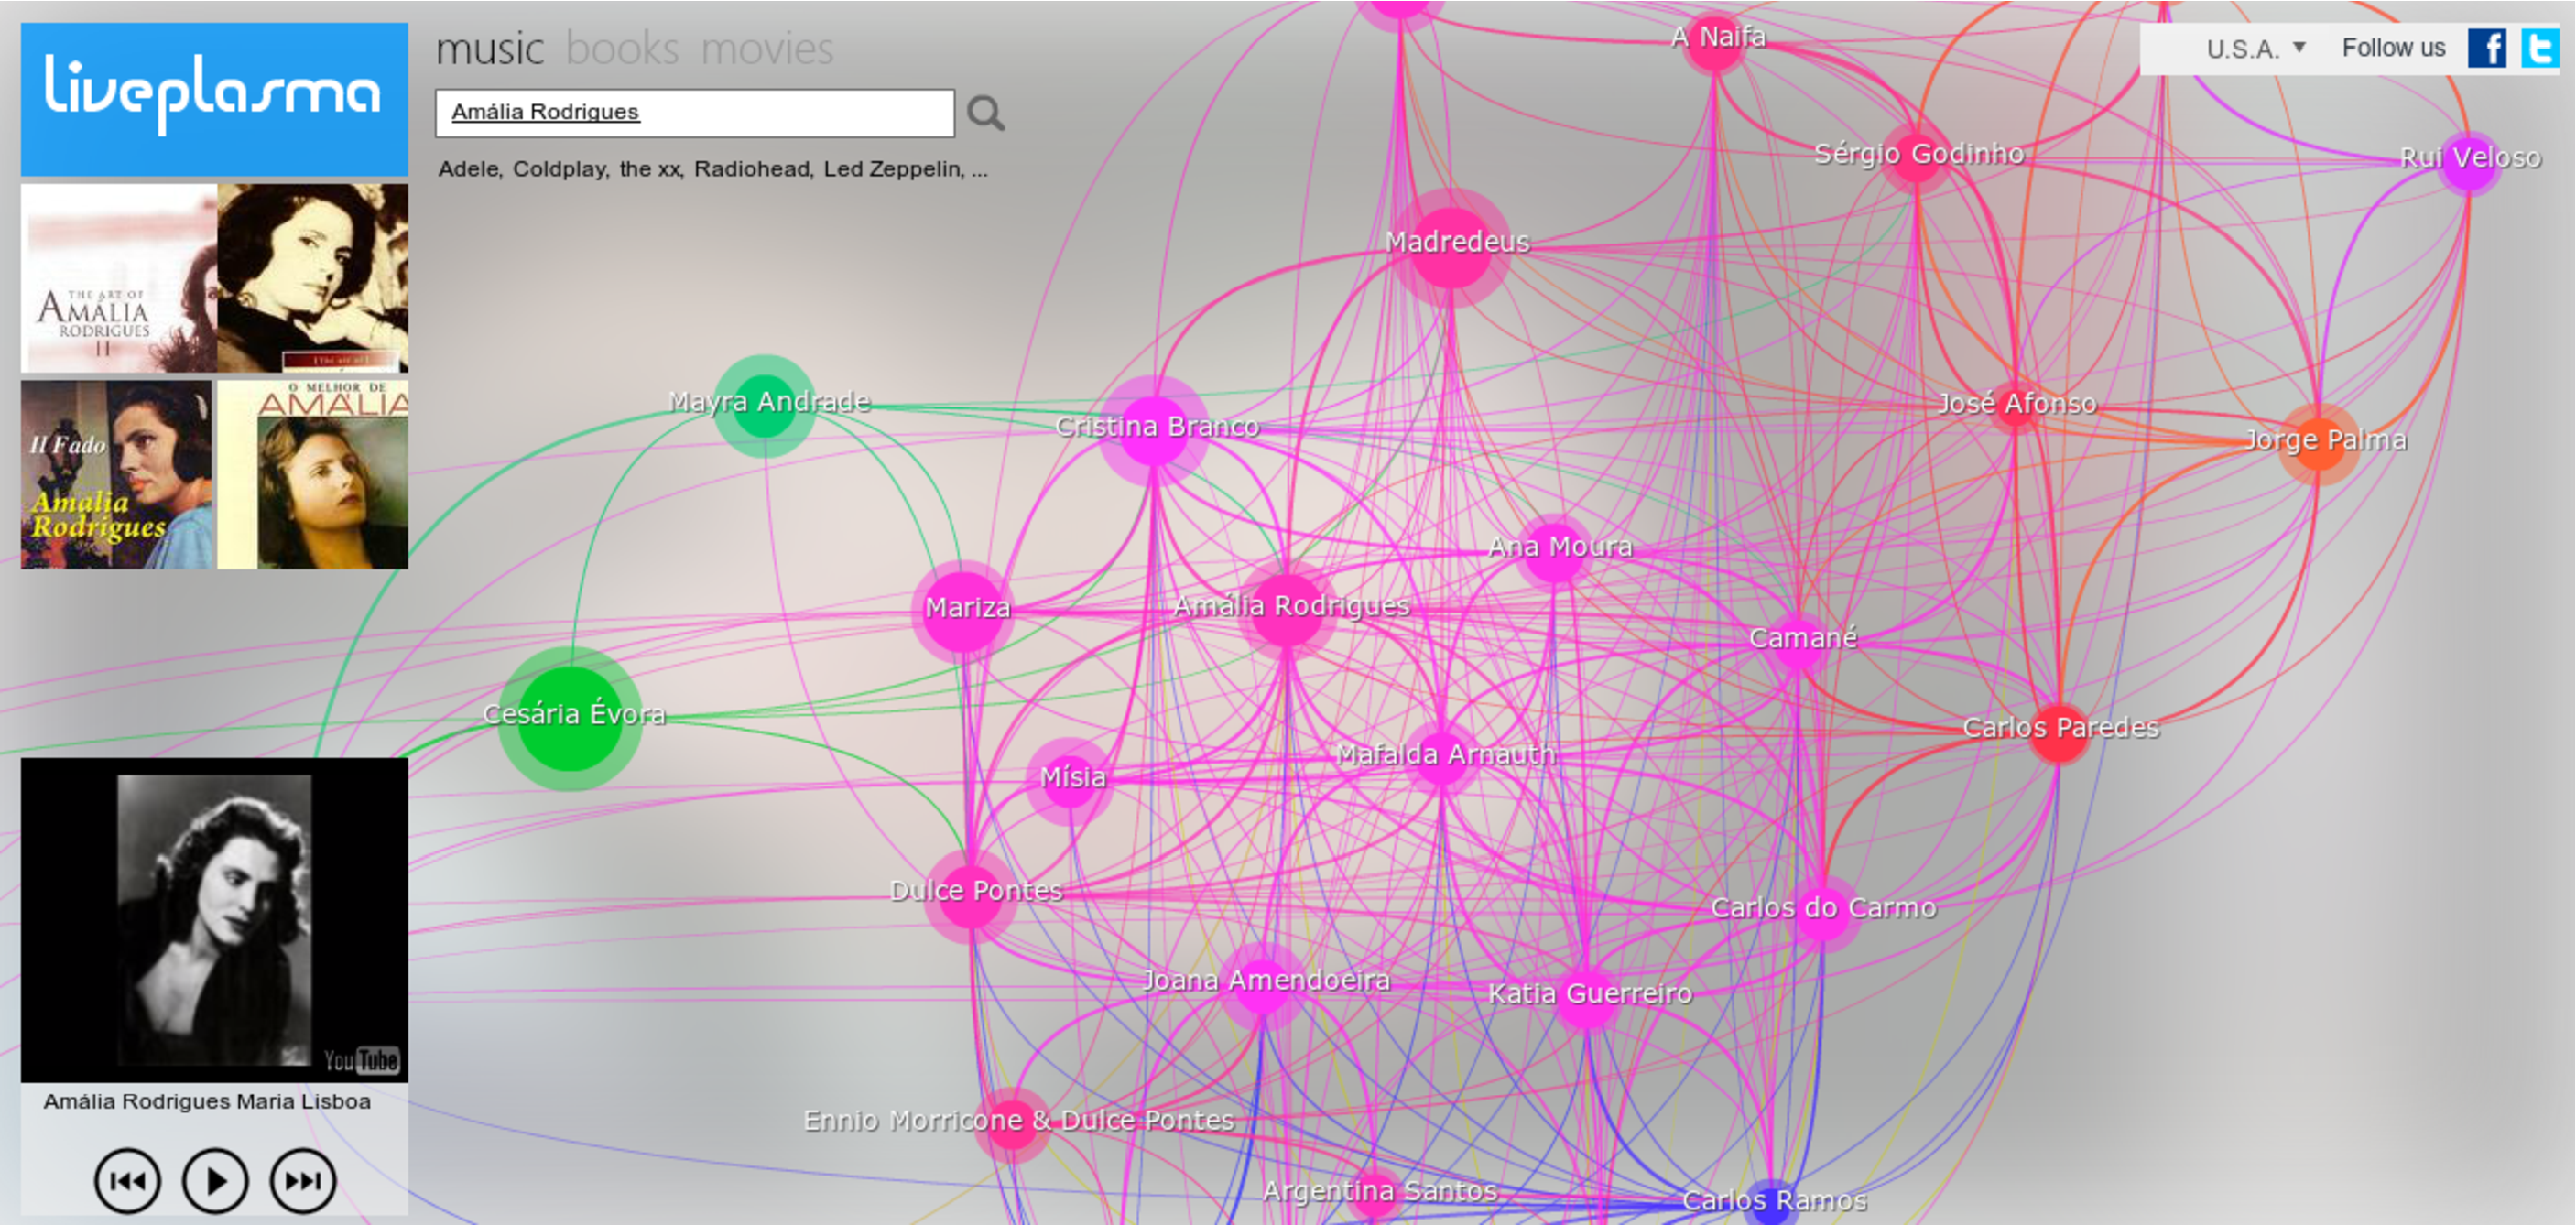
\includegraphics[width=\textwidth]{liveplasma.pdf}
  \end{center}
  \caption{liveplasma: resultado da pesquisa "Amália Rodrigues". Canto superior esquerdo: álbums da artista; Canto inferior esquerdo: \emph{mini-player} do youtube}.
  \label{fig:sota_liveplasma}
\end{figure}

Na figura \ref{fig:sota_liveplasma} podemos ver o resultado de uma pesquisa.
É possível ver a grelha com os álbums que o artista lançou, que redirecionam o utilizador para a Amazon\footnote{http://amazon.com} para comprar os álbums e um \emph{mini-player} que começa a reproduzir uma música do artista diretamente do Youtube.

É possível controlar que músicas são reproduzidas de uma forma interessante: ao passar o rato por cima de um nó, aparece dois botões que permitem reproduzir música só do próprio artista (botão \emph{only}) ou só de artistas parecidos (botão \emph{similar}).
É possível ver esses botões na figura \ref{fig:sota_liveplasma2}

\begin{figure}[tb]
  \begin{center}
    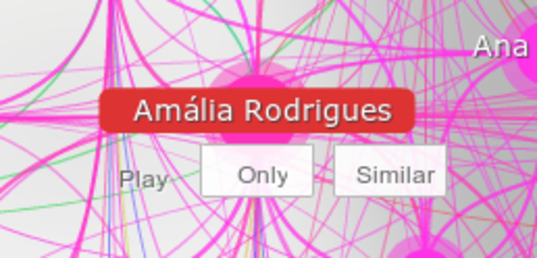
\includegraphics[]{liveplasma2.pdf}
  \end{center}
  \caption{liveplasma: interface para reprodução de música. Botão \emph{similar} reproduz músicas de artistas parecidos; Botão \emph{only} só reproduz músicas do artista pesquisado.}
  \label{fig:sota_liveplasma2}
\end{figure}

\subsubsection{Prós} % (fold)
\label{ssub:liveplasma_pros}

Os aspectos interessantes desta ferramenta são:

\begin{itemize}
  \item Links para compra dos álbums
  \item Reproduzir músicas de artistas semelhantes
\end{itemize}

% subsubsection pros (end)

\subsubsection{Contras} % (fold)
\label{ssub:liveplasma_contras}

O grafo desenhado é bastante confuso quando existem muitos nós com muitas ligações.
Isto acontece quando existem muitos artistas semelhantes.
Para além disso, são atribuídas cores aos nós que devem identificar o grau de parecença entre os artistas.
No entanto não existe nenhum tipo de informação que explique qual o seu verdadeiro significado ao utilizador, assim como também não existe uma explicação das ligações entre os nós.

É também de notar que o tamanho dos nós é diretamente proporcional à popularidade dos artistas respectivos, mas mais uma vez, este tipo de informação não é dada ao utilizador.

Outra falha a apontar é o facto de não se conseguir distinguir o nó de pesquisa dos restantes resultados em \ref{fig:sota_liveplasma} por exemplo.

% subsubsection contras (end)

\subsubsection{Resumo} % (fold)
\label{ssub:liveplasma_resumo}

Em suma, o liveplasma é usável, mas peca por ter muitas cores e ligações que tornam a experiência do utilizador ainda mais difícil do que a tradicional apresentação em lista ou grelha.

% subsubsection resumo (end)

% subsection projeto_1 (end)

\subsection{audiomap.tuneglue.net} % (fold)
\label{sub:projeto_2}



\subsubsection{Prós} % (fold)
\label{ssub:audiomap_pros}

% subsubsection pros (end)

\subsubsection{Contras} % (fold)
\label{ssub:audiomap_contras}

% subsubsection contras (end)

\subsubsection{Resumo} % (fold)
\label{ssub:audiomap_resumo}

% subsubsection resumo (end)

% subsection projeto_2 (end)

\subsection{Discovr.info} % (fold)
\label{sub:projeto_3}


% subsection projeto_3 (end)

% section projetos_relacionados (end)


\section{Resumo ou Conclusões}

